\documentclass[11pt,a4paper]{article}
\usepackage[a4paper,margin=25mm]{geometry}
\setcounter{tocdepth}{4}
\usepackage[utf8]{inputenc}
\usepackage[T1]{fontenc}
\usepackage{lmodern}
\usepackage{amsmath}
\usepackage{amsthm}
\usepackage{amssymb}
\usepackage{mathrsfs}
\usepackage{amsfonts}
\usepackage{stmaryrd}
\usepackage{xfrac}
\usepackage{dsfont}
\usepackage{fancybox}
\usepackage{fancyref}
\usepackage{multicol}
\usepackage{graphicx}
\usepackage{wrapfig}
\usepackage{textcomp}
\usepackage{mathrsfs}
\usepackage[svgnames]{xcolor}
\usepackage{color}
\usepackage{listings}
\usepackage{tikz-cd}
\usepackage[colorlinks=true, linkcolor=black, urlcolor=blue, citecolor=black, anchorcolor=blue, pdfencoding=auto, psdextra]{hyperref}
\usepackage{cleveref}
\usepackage{comment}
\usepackage{caption}
\usepackage{shuffle}
\usepackage{multirow}
\usepackage{appendix}
\usepackage{fdsymbol}
\usepackage{float}
\usepackage{algorithm}
\usepackage[noend]{algpseudocode}
\usepackage{qcircuit}

\newcommand{\HRule}{\rule{\linewidth}{0.5mm}}
\newcommand{\Dyck}[1]{\textsc{Dyck$_{#1}$}}
\newcommand{\FA}[1]{\textsc{FindAny$_{#1}$}}
\newcommand{\FFL}[1]{\textsc{FindFixedLength$_{#1}$}}
\newcommand{\FFP}[1]{\textsc{FindFixedPos$_{#1}$}}
\newcommand{\FALM}[1]{\textsc{FindAtLeftMost$_{#1}$}}
\newcommand{\FARM}[1]{\textsc{FindAtRightMost$_{#1}$}}
\newcommand{\FF}[1]{\textsc{FindFirst$_{#1}$}}
\newcommand{\Null}{\textsc{Null}}

\newcommand{\hered}[1]{\paragraph*{Induction:}{#1}}
\newcommand{\init}[1]{\paragraph*{Initialization:}{#1}}
\newcommand{\IH}[1]{\paragraph*{Induction Hypothesis:}{#1}}
\newcommand{\Conc}[1]{\paragraph*{Conclusion:}{#1}}
\newcommand{\remark}[1]{\paragraph*{Remark:}{#1}}
\newcommand{\observation}[1]{\paragraph*{Observation:}{#1}}
\newcommand{\notation}[1]{\paragraph*{Notation:}{#1}}
\newcommand{\property}[1]{\paragraph*{Property:}{#1}}
\newcommand{\ket}[1]{\ensuremath{|#1\rangle}}
\newcommand{\metersymbol}[1]{\begin{tikzpicture}[scale=#1]
    \draw (.8, 0) arc (0:180:.8);
    \draw[->] (0, 0) -- (1, 1);
\end{tikzpicture}
    }

\renewcommand{\comment}[1]{}
\newcommand\blfootnote[1]{%
    \begingroup
    \renewcommand\thefootnote{}\footnote{#1}%
    \addtocounter{footnote}{-1}%
    \endgroup
}

\theoremstyle{definition}
\newtheorem{definition}{Definition}
\newtheorem{proposition}{Proposition}[definition]

\theoremstyle{plain}
\newtheorem{theorem}{Theorem}[section]
\newtheorem{corollary}{Corollary}[theorem]
\newtheorem{lemma}{Lemma}[theorem]

\theoremstyle{definition}
\newtheorem{conjecture}{Conjecture}[definition]
\newtheorem{cproof}{Proof Corollary}[theorem] 
\newtheorem{lproof}{Proof Lemma}[theorem]
\newtheorem{tproof}{Proof Theorem}[section]

\begin{document}

\begin{titlepage}
    \begin{sffamily}
        \begin{center}

            \textsc{\LARGE École Normale Supérieure de Lyon}\\[0.5cm]
            \textsc{\LARGE Latvijas Universitāte} \\[1cm]

            \begin{minipage}[c]{.46\linewidth}
                \hspace{-2cm}
                \includegraphics[width=9.5cm]{illustration/Logo_ENS_Lyon.png}
            \end{minipage}
            \hfill%
            \begin{minipage}[c]{.46\linewidth}
                \centering
                \includegraphics[width=8cm]{illustration/Faculty_of_Computing_University_of_Latvia-1536x619-1.png}
            \end{minipage}\\[1cm]

            \textsc{\Large M1 Internship Repport}\\[1cm]

            \HRule \\[0.4cm]
            \textsc{\huge Complexity of recognizing Dyck languages
                of bounded height with quantum query algorithms.}
            \HRule \\[1cm]

            \begin{center}
                \textbf{Key words:} \textit{Quantum query complexity, Dyck words,
                    Quantum algorithms, regular languages, star free languages,
                    adversary methods.}
            \end{center}

            \vfill

            \begin{figure}[h!]
                \begin{center}
                    \begin{tikzpicture}[scale=.8]
                        \node[inner sep=0pt] (charlie) at (0, 0)  {\includegraphics[width=.42\textwidth]{illustration/3156684380_2_2_vxsNaxNA.jpg}};
                        \node[inner sep=0pt] (knuth) at (6.5, -1) {\includegraphics[width=.16\textwidth]{illustration/knuth.png}};
                        \node[inner sep=0pt] (grover) at (10, -1) {\includegraphics[width=.145\textwidth]{illustration/grover.jpeg}};
                        \node (textknuth) at (6.5, 2.79) {Finding Charlie};
                        \node (textknuth) at (6.5, 2.47) {will take};
                        \node (textknuth) at (6.5, 2.07) {a linear time...};
                        \draw[rounded corners=4mm] (6, 1.7) -- (4.7, 1.7) -- (4.7, 3.2) -- (8.3, 3.2) -- (8.3, 1.7) -- (7, 1.7);
                        \draw (6, 1.7) -- (6.7, 1.3) -- (7, 1.7);
                        Most people do not know what they are selling so just search a general name like “singer”  \node (textgrover) at (10, 2.15) {Sure of that?};
                        \draw[rounded corners = 2.5mm] (9.5, 1.7) -- (8.5,1.7) -- (8.5, 2.6) -- (11.5, 2.6) -- (11.5, 1.7) -- (10.5, 1.7);
                        \draw (9.5, 1.7) -- (9.8, 1.3) -- (10.5, 1.7);
                    \end{tikzpicture}
                \end{center}
                \caption{Historical discussion between Knuth and Grover.}
            \end{figure}
            \vfill

            % Author and supervisor
            \hspace{-0.8cm}
            \begin{minipage}{0.4\textwidth}
                \begin{flushleft} \large
                    \emph{Student:} \\
                    Maxime \textsc{Cautrès}\\
                \end{flushleft}
            \end{minipage}
            \hspace{3cm}
            \begin{minipage}{0.4\textwidth}
                \begin{flushright} \large
                    \emph{Supervisor:}\\
                    Andris \textsc{Ambainis}\\
                    Kamil \textsc{Khadiev}\\
                \end{flushright}
            \end{minipage}

            \vspace*{0.5cm}
            % Bottom of the page
            {\large   May the 2nd 2022 -  July the 22th 2022}
        \end{center}
    \end{sffamily}
\end{titlepage}

\tableofcontents

\newpage

\section{Introduction}

\subsection*{Context of the internship}

As part of the \href{http://informatique.ens-lyon.fr/en/academic-programs/master/m1}{first year of Master} at the
\href{http://www.ens-lyon.fr/en/}{École Normale Supérieure de Lyon},
I was able to do a 12 weeks research internship in a laboratory.

My research for an internship in Quantum Algorithmic had brought me to
the \href{https://www.lu.lv/en/studies/faculties/faculty-of-computing/}{Faculty of Computing}
at the \href{https://www.lu.lv/}{University of Latvia}
and my supervisor \href{http://home.lu.lv/~ambainis/}{Andris Ambainis}. My research also
brought me to discuss with \href{https://kpfu.ru/Kamil.Hadiev?p_lang=2}{Kamil Khadiev}
from \href{https://eng.kpfu.ru/}{Kazan Federal University} who became my co-supervisor.
We discussed by email to find an interesting subject of research on which I
liked to work on. I thank them for their help, their supervision and the time they
gave to me during this 12 weeks.

During the internship, I have been integrated to the life of the
\href{https://quantum.lu.lv/}{Center for Quantum Computing Science}.
I thanks members of the team for the great discussions we had after
the seminar.

I also want to thank \href{https://perso.ens-lyon.fr/omar.fawzi/}{Omar Fawzi} for
having introduced me to quantum computing and its fascinating possibilities.

The team's research area is quantum algorithms and complexity theory. More precisely,
the team works on establishing new quantum algorithms with better complexity and proving
new bounds to the quantum complexity for many different types of problem belonging
from graph theory to cryptography passing by language recognition theory. My work on
the recognition of restricted Dyck words integrated itself great in the team work as it
has already been studied by the team for few years \cite{art:2DGrid} and further by
Kamil Khadiev \cite{DBLP:conf/uc/KhadievK21}.

My internship, named "Complexity of recognizing Dyck language with a
quantum computer", had for goal to reduce the gap between the lower and the upper bound for
the quantum query complexity of recognizing Dyck words of bounded height. The best
known lower and upper bounds are describe in \cite{art:2DGrid} by Andris Ambainis team.

In the end of the introduction, the field of research will be presented more precisely.
After that, technical preliminaries, which are useful to understand the
current and the new results, will be detailed. Finally, the last two sections present my
new results for the quantum query complexity of bounded height Dyck word and the different
tries to improve both upper and lower bounds.

\subsection{History of quantum computing}

The history of quantum computing has started in 1980 when Paul Benioff, an american physicist,
proposed a quantum mechanical model of Turing machines \cite{art:paulbenioff}.
His machine uses some properties of the matter that has been discovered by quantum physicists.
After that, some computer scientists suggested that the quantum model of Turing machines may be
more expressive that the classical model. Few years after, the first bricks of the quantum circuit
have been introduced by Richard Feynman \cite{art:feymann}. The first quantum computers have started
to arrived in the middle of 1990s. During the last 20 years, the funds given to the creation of
the first quantum computer have skyrocketed, as the number of start-ups and companies dedicated to it.
This emulation has made from the quantum computer field one of the most active field of research today.
On the algorithmic side, the first astonishing result is the algorithm designed by Peter Shor (1994)
\cite{art:shor}. The algorithm improves a lot the complexity of factorizing integers, enough to break our
cryptographic protocols when quantum computer will be powerful enough. Since 1994, the
quantum algorithm area has evolved almost independently from the quantum computers and
has developed many beautiful theories and interesting results. But first, how does a quantum
circuit works?

\subsection{The quantum circuit, and quantum query model and complexity}

In classical computer science, the piece of information is represented with
0 and 1. This two states can be easily obtained using electricity because 0
can be represented by 0V and 1 by 5V, it is easy to propagate electricity
through wires and to stock its level into capacitor. Moreover a little piece
of hardware, named transistor, has allowed to do some computations using logical
gates which once include in a complex machine create our so-called "computers".

For quantum computers, the story isn't so different. First, the 0 and 1 are
now represented using particles like electrons or photons. For example,
an electron with a spin of $+\frac{1}{2}$ (noted \ket{1}, pronounced ket 1) represents a 1 and
an other one with a spin of $-\frac{1}{2}$ (noted \ket{0}, pronounced ket 0) represents a 0.
But the use of particles is motivated by their properties and mainly by
a quantum property called superposition. A quantum state is not only \ket{0}
or \ket{1}, but can be both in the same time, i.e.
$\lambda_0 \ket{0} + \lambda_1 \ket{1}$ for every $\lambda_{0, 1} \in \mathbb{C}$
such that $\vert\lambda_0\vert^2+\vert\lambda_1\vert ^2=1$. A quantum bit,
called qubit, correspond to a quantum state that is a superposition of two
value. As before, the computations are done by gates, here
quantum gates, which transform the quantum state of a qubit into another
quantum state.
At the end, to get the result of a computation, it is mandatory to measure the
state of the quantum system, which breaks the quantum superposition. A quantum
state of $n$ qubits can be represented with a vector in a $2^n$
dimensional space whose norm is equal to 1, and a quantum gate by a linear
unitary transformation on a $2^n$ dimensional space. A transformation is said
unitary if it preserved the lengths.

\paragraph*{A quantum circuit} is a precise configuration of quantum gates
on a finite number of qubits. The following \autoref{fig:quantum_circuit_examle}
represents the quantum circuit that computes a uniform randomize on $\{0, 1\}^n$.

\begin{figure}[h!]
    \begin{minipage}{.30\textwidth}
        \centering
        $
            \Qcircuit @C=.8em @R=1em {
            \mbox{$n$ \textrm{entries}} &     &                              &     & \mbox{$n$\ \textrm{outputs}}    \\
            \lstick{\ket{0}} & \qw & \multigate{2}{H^{\otimes n}} & \qw & \meter & \cw\\
            \vdots & & \ghost{H^{\otimes n}} & \qw & \vdots &\\
            \lstick{\ket{0}}& \qw & \ghost{H^{\otimes n}} & \qw & \meter & \cw\\
            }$
    \end{minipage}
    \hfill
    \begin{minipage}{.65\textwidth}
        \textbf{Legend:}

        $ \bullet \
            \Qcircuit @C=1em @R=1em {
            & \qw & & \cw \\
            }$ are respectively a quantum wire and a classical wire.

        $\bullet \ \Qcircuit @C=.4em @R=.4em {
            & \gate{H^{\otimes n}} \\
            }$ is the Hadamard's gates on each input qubit.

        $\bullet \ \Qcircuit @C=.4em @R=.4em {
            & \meter \\
            }$ is the measure of 1 qubit in the algorithm.
    \end{minipage}
    \caption{A quantum circuit computing the uniform random on $\{0, 1\}^n$. }
    \label{fig:quantum_circuit_examle}
\end{figure}

\paragraph*{The quantum query circuit} is a quantum circuit used to
compute function on an entry $x=x_1 \ldots x_N$ that belongs to an entry space.
The black box model \cite{black_box_andris} of a quantum query circuit is composed of
an input state $\ket{\psi_ {start}}$ and a sequence
$U_0, Q, U_1, \ldots, Q, U_T$ of linear unitary transformations such that $\ket{\psi_{start}}$ and all $U_i$
do not depend on entry $x$ unlike the $Q_i$ which depend on $x$. The quantum state
$\ket{\psi_ {start}}$ belongs to a $d$-dimensional space generated
by $\ket{1}, \ket{2},\ldots, \ket{d}$.  To define $Q$, the basis vectors first need to
be renamed from $\ket{1},\ldots, \ket{d}$ to $\ket{i, j}$ with
$i \in \llbracket 0, N\rrbracket$ and $j \in \llbracket1, d_i \rrbracket$ for some
$d_i$ such that  $d_1 + d_2 + \ldots + d_N = d$. Next, $Q$ is define such that

\[Q(\ket{i, j}) := \left\{
    \begin{array}{ll}
        \ket{0, j}  & \textrm{if\ } i = 0                           \\
        \ket{i, j}  & \textrm{if\ } i > 0 \ \textrm{and\ } x_i = 0  \\
        -\ket{i, j} & \textrm{if\ } i > 0 \ \textrm{and\ } x_i = 1.
    \end{array}
    \right.  \]

The gates $Q$ are doing the queries to input $x$ by flipping some of the vectors.
Finally, to get the output of the quantum query algorithm it is necessary to
measure the output. A quantum query algorithm can the summarized with the following
quantum circuit.

\begin{figure}[h!]
    \centering
    $
        \Qcircuit @C=.8em @R=1em {
        \lstick{\vdots} & \qw & \multigate{2}{U_0}  & \multigate{2}{Q} & \multigate{2}{U_1} & \qw &  & &  \multigate{2}{Q} & \multigate{2}{U_T}&\multigate{2}{\metersymbol{.2}} & \cw\\
        &\lstick{\ket{\psi_{start}}} qw & \ghost{U_0} & \ghost{Q} & \ghost{U_1} & \qw & \cdots & & \ghost{Q} & \ghost{U_T} & \ghost{\metersymbol{.2}}& \cw\\
        \lstick{\vdots}& \qw & \ghost{U_0} & \ghost{Q}  & \ghost{U_1} & \qw & & &\ghost{Q} &\ghost{U_T}&\ghost{\metersymbol{.2}}& \cw \\
        }$
    \caption{Structure of a quantum query algorithm.}
    \label{fig:quantum_query_algorithm_structure}
\end{figure}

\paragraph*{The quantum query complexity} of an algorithm corresponds to the number of calls to the $Q$ gate. Often, this number of calls
is depending on the size of the entry. The quantum query complexity of a problem corresponds to the highest possible bound for which it is
certain there is no quantum query algorithm with a lower quantum query complexity solving the problem.

\subsection{Dyck Languages of height $k$}

First, the Dyck language corresponds to the set of correct and balanced words of parenthesis.
Often, computer scientist used another more graphical and convenient definition where
parenthesis words are replaced with discrete paths onto a 2D space. Indeed, every path starts
at coordinate $(0, 0)$ and is composed of 2 types of steps: The first one is an increasing step
that is represented  by adding to the end of the current path the vector $\overrightarrow{ (1,1)}$.
The second one is an decreasing step, it works similarly but the add vector is $\overrightarrow{ (1,-1)}$.
Moreover, to be a Dyck path, the path should start with an increasing step, it should never cross
the abscise axis and it should finish on it. A Dyck word of length 12 is presented in \autoref{fig:dyck_word}.
The Dyck language is a context free language as it can easily be recognized using a context
free grammar. The work done by Andris Ambainis' team \cite{art:2DGrid} focus on a restriction
on Dyck language with bounded height $k$. More precisely, a Dyck word is of height at most $k$ if, in every
of its prefix, the difference between the number of opening and closing parenthesis does not
exceeds $k$. In the path representation, a path is said to be of height at most $k$ if the path
never cross the line $y = k$. \autoref{fig:dyck_word} illustrates two different Dyck words with
only one of height at most 3. The restricted Dyck language with bounded height $k$ is noted \Dyck{k}
and is interesting because it belong to the already well studied class of star
free languages (Detail in \autoref{ssec:starfree}).

\begin{figure}[h!]
    \centering
    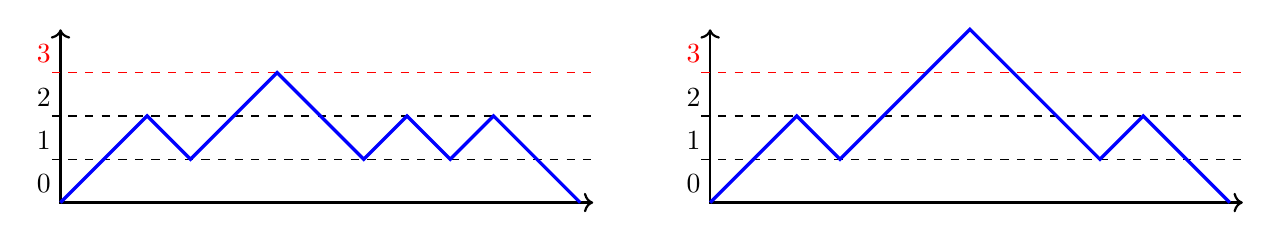
\begin{tikzpicture}[scale=.55]
        \draw[<->, thick] (0, 4) -- (0, 0)  -- (12.3, 0);
        \draw[dashed] (-.2, 1) -- (12.3, 1);
        \draw[dashed] (-.2, 2) -- (12.3, 2);
        \draw[dashed, red] (-.2, 3) -- (12.3, 3);
        \draw[blue, very thick] (0, 0) -- (2, 2) -- (3, 1) -- (5, 3) -- (7, 1) -- (8, 2) -- (9, 1) -- (10, 2) -- (12, 0);
        \draw (0, 0) node[above left] {0};
        \draw (0, 1) node[above left] {1};
        \draw (0, 2) node[above left] {2};
        \draw[red] (0, 3) node[above left] {3};

        \draw[<->, thick] (15+0, 4) -- (15+0, 0)  -- (15+12.3, 0);
        \draw[dashed] (15+-.2, 1) -- (15+12.3, 1);
        \draw[dashed] (15+-.2, 2) -- (15+12.3, 2);
        \draw[dashed, red] (15+-.2, 3) -- (15+12.3, 3);
        \draw[blue, very thick] (15+0, 0) -- (15+2, 2) -- (15+3, 1) -- (15+6, 4) -- (15+9, 1) -- (15+10, 2) -- (15+12, 0);
        \draw (15+0, 0) node[above left] {0};
        \draw (15+0, 1) node[above left] {1};
        \draw (15+0, 2) node[above left] {2};
        \draw[red] (15+0, 3) node[above left] {3};
    \end{tikzpicture}
    \caption{\textbf{On the left}, a valid Dyck word of height at most 3. \textbf{On the right}, an invalid Dyck word of height at most 3.}
    \label{fig:dyck_word}
\end{figure}

\subsection{State of the art}
This state of the art is not too precise as the understanding of the
bibliography took almost the first half the internship and is
more detail in \autoref{sec:preli}. First, few years ago Aaronson,
Grier and Schaeffer \cite[2019]{trichotomy_not_andris} worked on quantum query complexity
of recognizing regular languages as they can model a lot of tasks. They
concluded that there are 3 different cases depending of the language:
\begin{itemize}
    \item $O(1)$ if it is sufficient to read constant number of letters at the beginning and the end.
    \item $\tilde{\Theta}(\sqrt{n})$ if a Grover's search\footnote{
              The Grover search is a quantum query algorithm that allows to
              search for a marked element in a set of $n$ elements, where $p$ of them are marked,
              with a quantum query complexity of $O(\sqrt{\frac{n}{p}})$.
          } is the best way to recognize the language. The tilde refers to the existence of a
          constant $c_{te}$ such that the quantum query complexity is
          equal to $\Theta \left(\sqrt{n}(\log_2(n))^{c_{te}}\right)$.
    \item $\Theta(n)$ if recognizing the language is the same as counting modulo some value that can
          be computed with $O(n)$.
\end{itemize}
Further more, it is proved that being in the second classes is equivalent to
being a star free language. Andris Ambainis' team decided to work on \Dyck{k} as this
language is a beautiful example of star free languages. In \cite[2020]{art:2DGrid},
the team focused on finding the value of $c_{te}$, the power of the logarithm, in order
to find the exact quantum query complexity.
They first proved by reduction that the quantum query complexity of \Dyck{k}
called $Q\left(\Dyck{k}\right)$ is in $\Omega\left(c^k\sqrt{n}\right)$ where $c$ is
a constant greater than 1. They also gave an algorithm for \Dyck{k} with a quantum
query complexity of $O\left(\sqrt{n}(\log(n))^{0.5k}\right)$. Since then, no better
lower bound or algorithm have been found.

\subsection{Goals of the internship}
The problem on the quantum query complexity of \Dyck{k} is still open, my internship
has for goal to reduce the gap between the lower bound and the best known algorithm.
My researches have been organized on two main axes:
\begin{itemize}
    \item \textbf{Increasing the lower bound.} To do this, it is necessary to understand the bibliography
          on the adversary method in order to try to find a new adversary with better property. An other
          way is to use already existing lower bounds and translates them to \Dyck{k} with reductions.
    \item \textbf{Lowering the upper bound.} It is sufficient to find new algorithms
          with a better quantum query complexity than the previous ones. As for lower bounds,
          reduction method can also provides interesting new upper bounds.
\end{itemize}
Finally, the overall goal would be to made the two bounds match in order to get the exact quantum
query complexity of \Dyck{k}.

\subsection{Results}

The main results of my internship are presented in \autoref{main_section}. The first
one is a small revision of the original quantum query algorithm that recognize
\Dyck{k} \cite{art:2DGrid} and the second one is a new quantum query algorithm
for \Dyck{2} and its modifications to improve more the already revised original
algorithm.

\section{Preliminaries}\label{sec:preli}
In order to understand from where comes the $\tilde{\Theta}(\sqrt{n})$ quantum
query complexity, it is mandatory to start by understanding the
Trichotomy theorem \cite{trichotomy_not_andris} and its dependency on Regular
languages and star free languages.
After that, to understand how to find a lower bounds, it is necessary to explore
the different adversary methods \cite{adversary_equivalence}.

\subsection{Quantum query for regular languages.}

In the article \cite{trichotomy_not_andris}, Aaronson, Grier and Schaeffer presented
a really interesting algebraic characterization of regular languages based on the
recognition by monoids and the syntactic congruence. This totally new to me definition
give me some hard time in order to understand it correctly.

\subsubsection{Regular languages}

Usually, the set of regular languages $\mathcal{R}$ on the alphabet $\Sigma$ is defined as the smallest
fixed point of the function F (the function that computes concatenations, unions, and Kleene stars)
including $\{\varnothing\} \cup \{\varepsilon\} \cup(\cup_{l\in\Sigma}\{l\})$
with F equal
\begin{align*}\label{eq:F}
    F(X) = & \{AB\  \forall (A,B)\in X^2\}                                                   \\
           & \cup \{A\cup B\ \forall (A,B) \in X^2 \}                                        \\
           & \cup \{A\cap B\ \forall (A,B) \in X^2 \}\ \texttt{\color{gray!50}$\#$ optional} \\
           & \cup \{A^*\ \forall A \in X \}.
\end{align*}

But here, the more convenient way to characterize regular language is with their
algebraic characterization. Indeed, a regular language is always a pre image of a subset
of a monoid under monoid homomorphism. A monoid is a 3-tuple of a set M, an
internal associative binary operation and finally the identity element associated to the
operation. A monoid homomorphism is a map from a monoid to another that preserve the
operation and the identity. Usually, to get the monoid representation of a regular
language, the first step is to compute the syntactical monoid. The syntactical monoid is
obtained by dividing $\Sigma^*$ by the following equivalence relation called syntactic
congruence
\[x \sim_L y \Leftrightarrow \forall (u, v) \in \left(\Sigma^*\right)^2, (uxv \in L \Leftrightarrow uyv \in L).\]
This equivalence relation is a congruence relation as the equivalence class can be multiplied
(i.e. if $x\sim_L y$ and $u \sim_L v$ then $xu \sim_L yv$). Now, it is necessary to get the monoid
homomorphism. For that it is sufficient to take the homomorphism that map an element to its
congruence class. Inside a congruence class, none or every element of the class is in $L$.
Indeed,  if $x$ is in $L$ and $x \sim_L y$ then for all
$(u, v)$ in $\left(\Sigma^*\right)^2, (uxv$ in $L \Leftrightarrow uyv$ in $L)$ thus
$x$ in $L$ implies $y$ in $L$ and finally as $x$ is in $L$ then $y$ is also in $L$.
Now, it is sufficient to prove that the syntactical monoid is of finite size.
{\color{red} ma be put the proof if time else say folklore.}

Finally, every regular language can be recognized by finite monoid.

\subsubsection{Star free languages}\label{ssec:starfree}

The set of star free languages is a really well studied subset of the regular languages.
Its definition differs a little from regular languages' one as the Kleene star is replace
by the complement operation (note $\overline{L}$). So star free languages are defined
as the smallest fixed point of the function F' (the function that computes concatenations, unions
and complements) and such that it includes
$\{\varnothing\} \cup \{\varepsilon\} \cup(\cup_{l\in\Sigma}\{l\})$.
This restriction does not imply that every star free language is finite. Indeed,
$\Sigma^*$ can be written $\overline{\varnothing}$. For example the language on
$\Sigma = \{1, 2, 3\}$ described with the regular expression $\Sigma^*20^*2\Sigma^*$ can be written
as following in the star free way
$\overline{\varnothing}2\overline{\overline{\varnothing}\Sigma{\setminus}\{0\}\overline{\varnothing}}2\overline{\varnothing}$.

As for regular languages, it exists an algebraic characterization for star free
languages. Let $M$ be a monoid, $M$ is said to be aperiodic if for every $x$ in
$m$ it exits a positive integer $n$ such that $x^n=x^n+1$. A theorem proved by
Schützenberger \cite{Schtzenberger1965OnFM} state that a language is recognized
by a finite aperiodic monoid if and only if if is star free.

Good examples of star free languages are the Dyck word languages with bounded heights.
It is first easy to have a finite automata that recognize Dyck word of height $k$ by
putting one state for each integer from 0 up to $k$. However, the belonging to the star
free regular languages is more delicate to prove. It has been done done by Italian
researcher in \cite[1978]{dyck_height_bound_star_free}.

\subsubsection{Trichotomy theorem}

\begin{theorem}[Aaronson, Grier and Schaeffer \cite{trichotomy_not_andris}]
    Every regular language has quantum query complexity
    \(0,\Theta(1), \tilde{\Theta}(\sqrt{n}),\) or \(\Theta(n) \)
    according to the smallest class in the following hierarchy that contains
    the language.
    \begin{itemize}
        \item Degenerate: One of the four languages \(\varnothing, \varepsilon, \Sigma^*\), or \(\Sigma^+\).
        \item Trivial: The set of languages which have trivial
              \footnote{A language $L$ is said to be trivial if and only if it exists 2 finite size alphabets
                  $L_1$ and $L_2$ such that $L = L_1 \Sigma^* L_2$.}
              regular expressions.
        \item Star free: The set of languages which have star-free regular expressions.
        \item Regular: The set of languages which have regular expressions.
    \end{itemize}
\end{theorem}

This theorem is really important as it give a good idea on the quantum query complexity
of many language recognitions. Moreover, the classes are now clearly defined so it is now
easier to know where is a problem compared to the classes in the introduction. However,
it does not give the exact quantum query complexity because for star free languages
the result is given using \(\tilde{\Theta}\). The $\tilde{\Theta}(\sqrt{n})$ means that
the quantum query complexity of any star free regular language is in
$\Theta(\sqrt{n}(\log_2(n))^p)$ for some $p$ a non negative constant.
As it is known that \Dyck{k} languages are star free, it is an interesting problem
to find the power of $\log_2(n)$ depending on the value of $k$.

\subsection{The bounds for \Dyck{k,n} problem}

The trichotomy theorem state that \Dyck{k,n} language has a quantum query complexity
in $\tilde{\Theta}(\sqrt{n})$. The $\Theta$ means that the best possible algorithm
is both a $\tilde{O}(\sqrt{n})$ and a $\tilde{\Omega}(\sqrt{n})$. So, a common method
to find the power of $\log_2(n)$ depending on $k$ is the squeeze theorem. More
precisely, the quantum query complexity of \Dyck{k, n} is trapped between a lower
and an upper bound for quantum query complexity. So it is possible to deduce
the quantum query complexity from an increasing sequence of lower bound and
a decreasing sequence of upper bound such that they share the same limit $l$ with $l$
equals to $Q(\Dyck{k,n})$. How to find this sequence ?
\begin{itemize}
    \item \textbf{For the lower bound sequence.} Some of the most important tools to compute
          lower bounds are called \textbf{quantum adversary methods} and have been invented by Ambainis
          \cite{andris_adversary_methode}. This tools can compute
          lower bounds more or less tight and some of this adversary methods have really
          useful property such as being compatible with a certain type of composition
          of problems. This lead to the \textbf{reduction methods} that can compute
          a lower bounds from different but easier problem's ones.
    \item \textbf{For the upper bound sequence.} The main method is to \textbf{find quantum
              query algorithms} that are more and more efficient. An other way is also
          \textbf{by reduction} to a more difficult problem with a
          good enough upper bound.
    \item \textbf{For the same limit.}
          The idea is to do an iterative process where each step improves successively
          each bound until only one will continue to be improved. Finally, both
          bounds may end up matching. However, before my internship, both \Dyck{k,n}'s
          lower and upper bounds where stuck to $\Omega\left(c^k\sqrt{n}\right)$ for some
          constant $c$ greater than 1 and $O\left(\sqrt{n}\left(\log_2(n)\right)^{0.5k}\right)$.
\end{itemize}


\subsubsection{Lower bound on the quantum query complexity of \Dyck{k, n}}

\paragraph*{\textbf{The quantum adversary methods:}}
This part as for goal to present some quantum adversary methods and their usages.

\subparagraph*{\textbf{The adversary method.}} The adversary method is a classical
way to prove lower bound in classical algorithmic. Indeed, the idea behind the classical
adversary is to prove that for every algorithm, it exist an entry such that the algorithm
cannot decide in less unit of complexity than the lower bounds. In general, during
the algorithm execution, the adversary modifies entry values that have not been already used
in order to increase the execution time. This classical adversary work great for classical
algorithm but is not really useable on  quantum algorithms.

\subparagraph*{\textbf{The super basic quantum adversary method.}}
In order to recognize a language it is mandatory to be able to distinguish between
a valid word $v$ and an invalid word $w$. So at the output of the quantum query
algorithm, the states $\ket{\psi^T_v}$ and $\ket{\psi^T_w}$ should be distinguishable thus
$\vert \langle \psi_v^T \vert \psi_w^T \rangle \vert < \frac{2}{3}$. How do they
will differs? The quantum query algorithm start with
$\ket{\psi^0_v} = \ket{\psi^0_w} = \ket{\psi_{start}}$. Moreover, the inner product
of both states isn't affected by $U_i$ gates because there are unitary. However, the $Q_i$
gates affect this inner product as the $Q_i$'s behaviors are depending on the input.
Let define the progress measure $\mathcal{P}$ such that
$\mathcal{P}(t) := \langle \psi_v^t \vert \psi_w^t \rangle$ where $\ket{\psi^t}$ represents
the state after $Q_t$. Let suppose it exists $d$ such that for all $0\leq t \leq T-1$,
$\vert \mathcal{P}(t+1)-\mathcal{P}(t)\vert \leq d$. It implies the following inequality
\[
    \mathcal{P}(T) = \underbrace{\mathcal{P}(0)}_{=1} + \sum_{i=0}^{T-1}\underbrace{\mathcal{P}(i+1)-\mathcal{P}(i)}_{\geq -d}  \geq \mathcal{P}(0) - T\times d.
\]
Moreover, $\mathcal{P}(T)$ should be lower than $\frac{2}{3}$ so it implies that
$1 - T\times d$ should also be lower than $\frac{2}{3}$ and finally that
$T$ should be a $O(\frac{1}{d})$. This give a general idea of how to determined
a lower bound but it isn't precise enough to get a theorem. In its courses,
Ryan O'Donnell \cite{Odonnel_course} explained a simple to understand adversary method called the super
basic adversary method. This adversary allow to compute a lower bound
by using the following method:

\begin{theorem}
    Let define $YES$ the set equal to $f^{-1}(accepted)$ and $NO$ the set
    equal to

    $f^{-1}(rejected)$. If it exist two subset $Y\subseteq YES$ and
    $Z \subseteq NO$ such that:
    \begin{itemize}
        \item For each $y$ in $Y$, there are at least $m$ strings $z$ in $Z$ with dist$(y,z)=1$.
        \item For each $z$ in $Z$, there are at least $m'$ strings $y$ in $Y$ with dist$(y,z)=1$.
    \end{itemize}
    Then the quantum query complexity $Q(f)$ is in  $\Omega(\sqrt{m m'})$.
\end{theorem}

The proof of the theorem can be found in \autoref{proof:advmethod}. More generally,
the method of an adversary define a process to find the lower $d$ possible. The
super-basic adversary method as its name let suggest is simple but does not give
a tight lower bounds. For this, the method should be more complicated which results
in longer days on the board to find the parameters of the methods.

Let f be the function whose quantum query complexity is unknown. The two adversary methods
are described as following:
\begin{itemize}
    \item \textbf{The Basic adversary method by Ambainis \cite{andris_adversary_methode}}
          \begin{theorem}
              Let define $YES$ the set equal to $f^{-1}(accepted)$ and $NO$ the set
              equal to

              $f^{-1}(rejected)$. Moreover, let $Y\subseteq YES$, $Z \subseteq NO$, and
              let $\mathcal{R} \subseteq Y\times Z$ be a set of "hard to distinguish" pairs, such that:
              \begin{itemize}
                  \item For each $y$ in $Y$, there are at least $m$ strings $z$ in $Z$ with $(y,z)$ in $\mathcal{R}$.
                  \item For each $z$ in $Z$, there are at least $m'$ strings $y$ in $Y$ with $(y,z)$ in $\mathcal{R}$.
              \end{itemize}
              Also, let define $\mathcal{R}_i$ as a restriction from $\mathcal{R}$ such
              that $(y, z)$ is in $\mathcal{R}_i$ if and only if $(y, z)$ is in $\mathcal{R}$
              and $y_i \neq z_i$.
              In addition,
              \begin{itemize}
                  \item For each $y$ in $Y$ and $i$, there are at most $l$ strings $z$ in $Z$ with $(y,z)$ in $\mathcal{R}_i$
                  \item For each $z$ in $Z$ and $i$, there are at most $l'$ strings $y$ in $Y$ with $(y,z)$ in $\mathcal{R}_i$
              \end{itemize}
              Then the quantum query complexity $Q(f)$ is in  $\Omega(\sqrt{\frac{m m'}{ll'}})$.
          \end{theorem}
    \item \textbf{The general adversary method by \cite{}}
\end{itemize}

\paragraph*{\textbf{The reduction method:}}
\begin{itemize}
    \item how does it work
    \item how does it translate to quantum query complexity
    \item the result for a lower bound on \Dyck{k,n}
\end{itemize}

\subsubsection{Best known algorithm to recognize \Dyck{k, n}}

\paragraph*{\textbf{How to reject a word from \Dyck{k,n}}}
\begin{itemize}
    \item recall for the height $height$
    \item $\pm$ $k+1$ strings, minimal ones
\end{itemize}

\paragraph*{\textbf{explaination why it is hard for $k > 1$}}
\begin{itemize}
    \item There is an infinit number of rejecting strings to search for
\end{itemize}

\paragraph*{\textbf{Andris ambainis team solution}}
\begin{itemize}
    \item Give an detailed explaination of the algorithm that are in the annexe
    \item explain why every part of the algorithm is important.
          \begin{itemize}
              \item the search on $d$
              \item the log search to have limited error.
              \item \FALM{k}
          \end{itemize}
    \item
\end{itemize}


\section{A better algorithm for \Dyck{k,n}}
\label{main_section}

\subsection{A better complexity analysis of the original algorithm}

In the article \cite{art:2DGrid}, Andris Ambainis's team gave a quantum query
algorithm to recognize $\Dyck{k}$ that uses $O(\sqrt{n}(\log_2(n))^{0.5k})$
quantum queries. But the quantum query complexity for $k=1$
($O\left(\sqrt{n\log_2(n)}\right)$) is not as good as a Grover's search
$O(\sqrt{n})$ which is sufficient (seen in \autoref{already_known}).
More precisely, the logarithmic search done by \FA{k+1} for $k=1$ is useless
as there is exactly one minimal $\pm 2$ -string. So, it is sufficient to
add a new initial case to \FA{k+1} for $k = 1$ in order to use a Grover search
for $00$ and $11$ in $1w0$ instead of \FFL{2}. This small revision has lowered
the quantum query complexity for $k=1$ of the function to $O(\sqrt{n})$ instead
of $O(\sqrt{n\log_2(n)})$. This gives the following algorithm for \FA{k}

\begin{algorithm}
    \caption{\FA{k}(l,r,s)}\label{alg:FA_prim}
    \begin{algorithmic}
        \Require $0 \leq l < r$ and $s \subseteq \{1,-1\}$
        \If{$k > 2$}
        \State \textbf{Find} $d$ in $\{2^{\lceil \log_2(k)\rceil }, 2^{\lceil \log_2(k)+1\rceil },\ldots,2^{\lceil \log_2(r-l)\rceil }\}$
        such that \\
        \hspace*{1cm} $v_d \gets $ \FFL{k}$(l,r,d,s)$ is \textbf{not} \Null
        \State \textbf{return} $v_d$ or \Null \ if none
        \Else
        \State \textbf{Find} $t$ in $\{l, l+1, \dots, r\}$ such that \\
        \hspace*{1cm} $v_t \gets$ \FALM{2}$(l,r,t,2,s)$ is \textbf{not} \Null
        \State \textbf{return} $v_t$ of \Null \ if none.
        \EndIf
    \end{algorithmic}
\end{algorithm}

The same improvements can be done on \FFP{k} because if $k = 2$ the logarithmic
search is useless. So \FFP{k} can be redefined as in
\textsc{Algorithm}\autoref{alg:ffp_better}. For $k=2$, the complexity is
lowered from $O(\sqrt{\log_2(l-r)})$ to $O(1)$.

\begin{algorithm}
    \caption{$\FFP{k}(l,r,t,s)$}\label{alg:ffp_better}
    \begin{algorithmic}
        \Require $0\leq l<r$, $l \leq t \leq r$ and $s \subseteq \{1, -1\}$
        \If{$k>2$}
        \State \textbf{Find} $d$ in $\{2^{\lceil \log_2(k)\rceil }, 2^{\lceil \log_2(k)+1\rceil },\ldots,2^{\lceil \log_2(r-l)\rceil }\}$
        such that \\
        \hspace*{1cm} $v_d \gets $ \FALM{k}$(l,r,t,d,s)$ is \textbf{not} \Null
        \State \textbf{return} $v_d$ or \Null \ if none
        \Else
        \ $v \gets $ \FALM{k}$(l,r,t,2,s)$ is \textbf{not} \Null
        \State \textbf{return} $v_d$ or \Null \ if none
        \EndIf
    \end{algorithmic}
\end{algorithm}

This small improvements on two initial cases improve the global
quantum query complexity of each subroutine and finally the quantum
query complexity for \Dyck{k}.

\begin{theorem}{\textbf{\Dyck{k}'s algorithm correctness}} \label{th:subroutine_correctness}
    The new definitions of \FA{} and \FFP{} do not change the behavior the original algorithm
    as other subroutines (\autoref{annex:complete_subroutine_dyck_kn}) stay unchanged.
\end{theorem}

\begin{tproof}
    The behavior of the \Dyck{k} algorithm with the new subroutines hasn't changed
    as \FA{} (resp. \FF{}) has the same sub-behavior on every entry than its
    former definition.

    \qed
\end{tproof}

\begin{theorem}{\textbf{\Dyck{k}'s subroutines complexity}} \label{th:subroutine_complexity}
    The quantum query complexity of \Dyck{k} algorithm's subroutines are the following.
    \begin{enumerate}
        \item $Q$(\Dyck{k}) = $O\left(\sqrt{n}(\log_2(n))^{0.5(k-1)}\right)$ \ for $k \geq 1$
        \item $Q$(\FA{k+1}$(l,r,s)$) = $O\left(\sqrt{r-l}(\log_2(r-l))^{0.5(k-1)}\right)$ \ for $k \geq 1$
        \item $Q$(\FFL{k+1}$(l,r,d,s)$) = $O\left(\sqrt{r-l}(\log_2(r-l))^{0.5(k-2)}\right)$ \ for $k \geq 2$
        \item $Q$(\FALM{k+1}$(l, r, t, d, s)$) = $\left\{
                  \begin{array}{ll}
                      O\left(\sqrt{d}(\log_2(d))^{0.5(k-2)}\right) & \textrm{for} \ k \geq 2 \\
                      O(1)                                         & \textrm{for} \  k = 1
                  \end{array}
                  \right.$
        \item $Q$(\FF{k}$(l,r,s, left)$) = $O\left(\sqrt{r-l}(\log_2(r-l))^{0.5(k-2)}\right)$ \ for $k \geq 2$
        \item $Q$(\FFP{k}$(l,r,t,s)$) = $\left\{ \begin{array}{ll}
                      O\left(\sqrt{r-l}(\log_2(r-l))^{0.5(k-2)}\right) & \textrm{for} \ k \geq 3 \\
                      O(1)                                             & \textrm{for} \ k = 2
                  \end{array}
                  \right.$
    \end{enumerate}
\end{theorem}

\begin{tproof}
    The idea is that only the $O\left(\sqrt{n}\right)$ comes from the initial
    case for $k = 1$ and that each of the $k-1$ level of the recursion increases
    the final quantum query complexity with a $O\left(\sqrt{\log_2(n)}\right)$
    factor. The $O\left(\sqrt{\log_2(n)}\right)$ factor is proven by Andris
    Ambainis' team in \cite{art:2DGrid} while the $O\left(\sqrt{n}\right)$
    for $k = 1$ comes from the new version of \FA{k} (\textsc{Algorithm}
    \autoref{alg:ffp_better}). The complete proof for the theorem is given
    in \autoref{proof:complexity_dyckkn}.

    \qed
\end{tproof}

Unfortunately, the improvements done on the initial cases of some of
the subroutines are not sufficient to get a significant improvement
for the quantum query complexity of \Dyck{k} algorithm. However,
they are sufficient to match the theoretical upper bound gave by
the reduction.

\subsection{A new algorithm for \Dyck{2}}
\label{subsection:dyck2n}

First, we would like to find an algorithm with a quantum query complexity
near to match the lower bound describes by Andris
Ambainis' team in \cite{art:2DGrid}, $\exists c > 1$ such that
$Q\left(\Dyck{k}\right)=\Omega\left(\sqrt{n}c^k\right)$. So the
searched algorithm may have a quantum query complexity of
$O\left(\sqrt{n}\right)$.

For $k=1$, the query complexity comes only from a call to Grover's search.
For $k=2$ it no more possible to search for every minimal
$\pm 3$-strings without a linear number of call to Grover's search. So in
order to keep the quantum query complexity in $O\left(\sqrt{n}\right)$,
the algorithm should do a constant number of calls to Grover's search.

For that, we define a new alphabet that can express every even length
binary string and that has convenient properties for a Grover's search.
Let $\mathcal{A} = \{a, b, c, d\}$ be the alphabet where $a$ corresponds
to 00, $b$ to 11, $c$ to 01, and $d$ to 10. Every string of size 2 has
its associated letter in $\mathcal{A}$ thus every even length bit string
is expressed in $\mathcal{A}^*$. This alphabet allows to prove more easily
the following theorem.

\begin{theorem}{\textbf{Substrings rejection for Dyck word of height at most 2.}}
    A word on the alphabet $\mathcal{A}$ embodies a Dyck word of
    height at most 2 if and only if it does not contain $aa, ac, bb,
        bd, cb, cd, da,$ or$ dc$ as a substring.
\end{theorem}

\begin{tproof}
    First, this alphabet $\mathcal{A}$ is important because each letter
    has a height variation in $\{-2, 0, 2\}$. Indeed, $a$ has a height
    variation of 2, $b$ of $-2$, $c$ of 0, and $d$ of 0.
    So, after each letter in a word, the current height will be even.
    Moreover, for a valid Dyck word of height at most 2, only 0 and 2
    are even and accessible heights. So after every
    letter in a word, the height will be 0 or 2 which are respectively
    the lower and the upper bound for the height.

    \begin{figure}[h!]
        \centering
        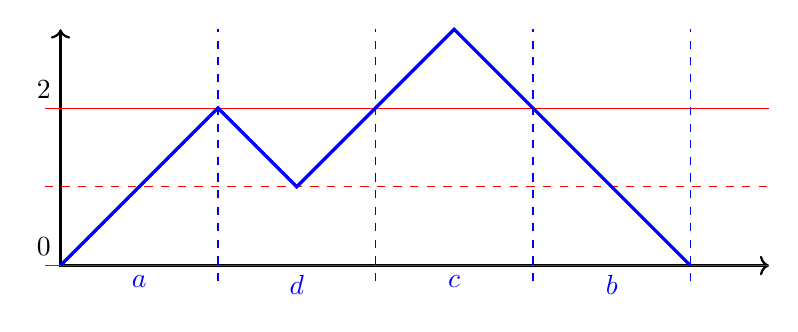
\begin{tikzpicture}
            \draw[<->, thick] (0, 3) -- (0, 0) -- (9, 0);
            \draw[dashed, red] (-.2, 1) --(9, 1);
            \draw[red] (-.2, 2) --(9, 2);
            \draw[red] (-.2, 0) --(9, 0);
            \draw[very thick, blue] (0, 0) -- (2, 2) -- (3, 1) -- (5, 3) -- (8, 0);
            \draw[blue, dashed] (2, -.2) -- (2, 3);
            \draw[blue, dashed] (4, -.2) -- (4, 3);
            \draw[blue, dashed] (6, -.2) -- (6, 3);
            \draw[blue, dashed] (8, -.2) -- (8, 3);
            \draw[blue] (1, 0) node[below] {$a$};
            \draw[blue] (3, 0) node[below] {$d$};
            \draw[blue] (5, 0) node[below] {$c$};
            \draw[blue] (7, 0) node[below] {$b$};
            \draw (0, 2) node[above left] {2};
            \draw (0, 0) node[above left] {0};
        \end{tikzpicture}
        \caption{Illustration of the letters of $\mathcal{A}$ using Dyck's representation.}
        \label{tikz:dyck2alphabet}
    \end{figure}

    This property is important as it implies that every substrings that cross a
    bounds uses at least two letters. So it may be possible that the belonging
    of some pairs of letters to a word implies its non belonging to \Dyck{2}.
    It founds out that $\mathcal{A}^2$ can be split into two sets described
    in \autoref{tab:partitionDyck2}.

    \begin{table}[htb]
        \centering
        \caption{Partition of $\mathcal{A}$ into $\mathcal{X}, \mathcal{V}$.}
        \label{tab:partitionDyck2}
        \begin{tabular}{|c|c|}
            \hline
            $\mathcal{X}$ & $aa$ $ac$ $bb$ $bd$ $cb$ $cd$ $da$ $dc$ \\
            \hline
            $\mathcal{V}$ & $ab$ $ad$ $ba$ $bc$ $ca$ $cc$ $db$ $dd$ \\
            \hline
        \end{tabular}


        \newpage
    \end{table}
    \begin{itemize}
        \item The set $\mathcal{X}$. First, every couple of letters which
              contains a $\pm 3$-string is in $\mathcal{X}$. This first
              condition explains the belonging of $aa, ac, dc, da, cb, bb,
                  bd, \textrm{and}\ cd $. Next, $cd$ and $dc$ belong to
              $\mathcal{X}$. Indeed, for any valid Dyck word of
              height at most 2, the current height is bounded between 0 and 2.
              After each letter the current height is even so both couple $cd$
              and $dc$ start and finish on the same bound. However, $cd$
              and $dc$ are going above and below the height at which they start
              so both are going outside off the bounds. Thus, a word which
              contains $cd$ or $dc$ can not be a Dyck Word of height a most 2.
              The \autoref{fig:rejectDyck2} shows each couple of $\mathcal{X}$.

              \begin{figure}[h!]
                  \centering
                  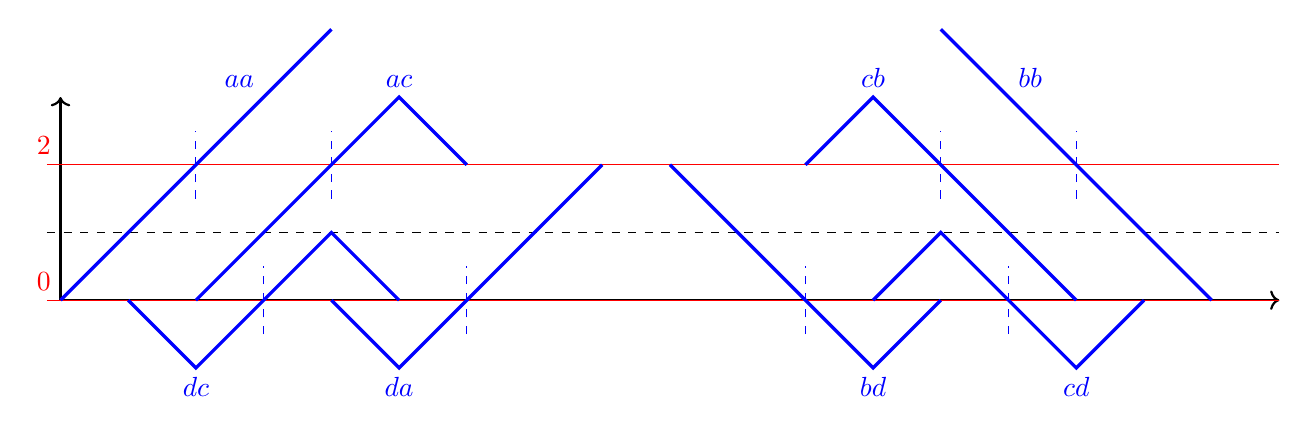
\begin{tikzpicture}[scale=.86]
                      \draw[<->, thick] (0, 3) -- (0, 0) -- (18, 0);
                      \draw[dashed] (-.2, 1) --(18, 1);
                      \draw[red] (-.2, 2) --(18, 2);
                      \draw[red] (-.2, 0) --(18, 0);
                      \draw[blue, very thick] (0, 0) -- (4, 4);
                      \draw[blue, very thick] (1, 0) -- (2, -1) -- (4, 1) -- (5, 0);
                      \draw[blue, very thick] (2,0) -- (5, 3) -- (6, 2);
                      \draw[blue, very thick] (4, 0) -- (5, -1) -- (8, 2);
                      \draw[blue, very thick] (9, 2) -- (12, -1) -- (13, 0);
                      \draw[blue, very thick] (12, 0) -- (13, 1) -- (15, -1) -- (16, 0);
                      \draw[blue, very thick] (11, 2) -- (12, 3) -- (15, 0);
                      \draw[blue, very thick] (13, 4)--(17,0);
                      \draw[red] (0, 2) node[above left] {2};
                      \draw[red] (0, 0) node[above left] {0};
                      \draw[blue] (2, -1) node[below] {$dc$};
                      \draw[blue] (5, -1) node[below] {$da$};
                      \draw[blue] (12, -1) node[below] {$bd$};
                      \draw[blue] (15, -1) node[below] {$cd$};
                      \draw[blue] (3, 3) node[above left] {$aa$};
                      \draw[blue] (5, 3) node[above] {$ac$};
                      \draw[blue] (12, 3) node[above] {$cb$};
                      \draw[blue] (14, 3) node[above right] {$bb$};
                      \draw[blue, dashed] (2, 2-.5) -- (2, 2.5);
                      \draw[blue, dashed] (3, -.5) -- (3, .5);
                      \draw[blue, dashed] (6, -.5) -- (6, .5);
                      \draw[blue, dashed] (4, 2-.5) -- (4, 2.5);
                      \draw[blue, dashed] (3, -.5) -- (3, .5);
                      \draw[blue, dashed] (11, -.5) -- (11, .5);
                      \draw[blue, dashed] (13, 2-.5) -- (13, 2.5);
                      \draw[blue, dashed] (14, -.5) -- (14, .5);
                      \draw[blue, dashed] (15, 1.5) -- (15, 2.5);
                  \end{tikzpicture}
                  \caption{Every 2 letters configuration that implies that a word, whom
                      a configuration is a substring, is not a Dyck word of height at most 2.}
                  \label{fig:rejectDyck2}
              \end{figure}

        \item The set $\mathcal{V}$. Every couple of $\mathcal{A}$ does not imply
              that the word is not a Dyck word of height at most 2 because some
              couple of $\mathcal{A}$ can fit inside the height bounds.
              The \autoref{fig:donotrejectDyck2} shows that every couple
              not in $\mathcal{X}$ (ie. $ab, ad, ba, bc, ca, cc, db,$ and $ dd$)
              can fit between heights 0 and 2.

              \begin{figure}[h!]
                  \centering
                  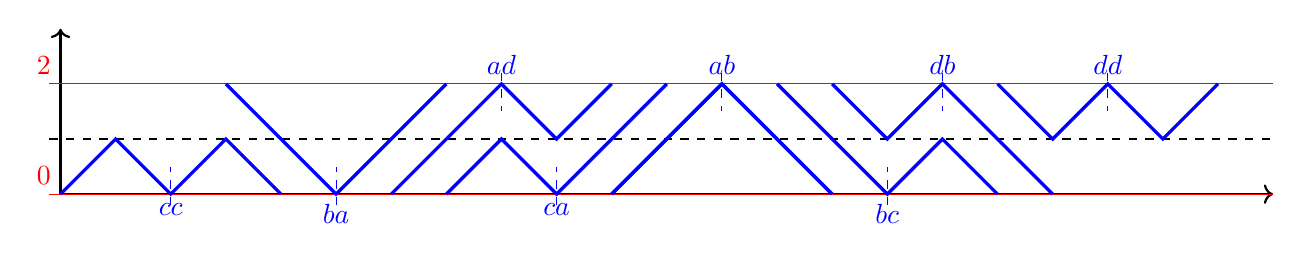
\begin{tikzpicture}[scale=.7]
                      \draw[<->, thick] (0, 3) -- (0, 0) -- (22, 0);
                      \draw[dashed] (-.2, 1) --(22, 1);
                      \draw[red] (-.2, 2) --(22, 2);
                      \draw[red] (-.2, 0) --(22, 0);
                      \draw[red] (0, 2) node[above left] {2};
                      \draw[red] (0, 0) node[above left] {0};
                      \draw[blue, very thick] (10, 0) -- (12, 2) -- (14, 0);
                      \draw[blue, very thick] (13, 2) -- (15, 0) -- (16, 1) -- (17, 0);
                      \draw[blue, very thick] (14, 2) -- (15, 1) -- (16, 2) -- (18, 0);
                      \draw[very thick, blue] (17 ,2) -- (18, 1) -- (19, 2) -- (20, 1) -- (21, 2);
                      \draw[blue, very thick] (10, 0) -- (12, 2) -- (14, 0);
                      \draw[blue, very thick] (11, 2) -- (9, 0) -- (8, 1) -- (7, 0);
                      \draw[blue, very thick] (10, 2) -- (9, 1) -- (8, 2) -- (6, 0);
                      \draw[blue, very thick] (7, 2) -- (5, 0) -- (3, 2);
                      \draw[very thick, blue] (4 ,0) -- (3, 1) -- (2, 0) -- (1, 1) -- (0, 0);
                      \draw[blue] (2, 0) node[below] {$cc$};
                      \draw[blue] (5, 0) node[below] {$ba$};
                      \draw[blue] (8, 2) node[above] {$ad$};
                      \draw[blue] (9, 0) node[below] {$ca$};
                      \draw[blue] (12, 2) node[above] {$ab$};
                      \draw[blue] (15, 0) node[below] {$bc$};
                      \draw[blue] (16, 2) node[above] {$db$};
                      \draw[blue] (19, 2) node[above] {$dd$};
                      \draw[blue, dashed] (2,-.2) -- (2, .5);
                      \draw[blue, dashed] (5, -.2) -- (5, .5);
                      \draw[blue, dashed] (9, -.2) -- (9, .5);
                      \draw[blue, dashed] (8, 2.2) -- (8, 1.5);
                      \draw[blue, dashed] (12, 2.2) -- (12, 1.5);
                      \draw[blue, dashed] (16, 2.2) -- (16, 1.5);
                      \draw[blue, dashed] (19, 2.2) -- (19, 1.5);
                      \draw[blue, dashed] (15, -.2) -- (15, .5);
                  \end{tikzpicture}
                  \caption{Every 2 letters configuration that
                      can be found in a valid Dyck word of height at most 2.}
                  \label{fig:donotrejectDyck2}
              \end{figure}
    \end{itemize}

    So, a word in $\mathcal{A}^*$ that has a substring in $\mathcal{X}$
    cannot be a Dyck word of height two. But does every non Dyck word of height
    at most 2 has a substring in $\mathcal{X}$?

    A word is not a Dyck word of height at most 2 if it include a $\pm 3$-string. But how are represented $\pm 3$-strings using the letters?
    There are 8 different cases which are 2 by 2 symmetrical so
    \autoref{fig:p3string} and \autoref{fig:p3string2piece} show only the
    cases for $+3$-strings. In \autoref{fig:p3string}, every $+3$-string of
    size 3 is include in $aa$ or $ac$ so it is sufficient to search for this
    two couples. In \autoref{fig:p3string2piece} every $+3$-string of length
    greater than 3 is composed of 2 minimal $+2$-strings. It implies that
    one must be a $a$ while the other must be $da$
    of $dc$. Because $da$ or $dc$ are rejecting substrings, it is sufficient
    to search for them.

    \begin{figure}[h!]
        \begin{minipage}{.35\textwidth}
            \centering
            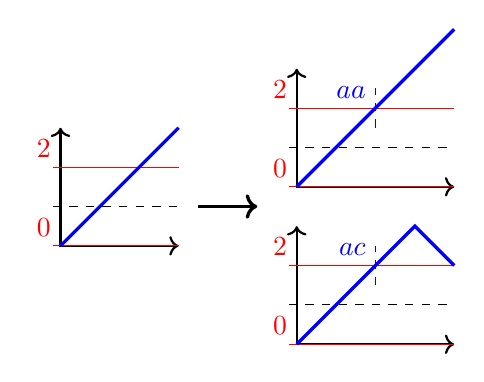
\begin{tikzpicture}[scale=.5]
                \draw[<->, thick] (0, 3) -- (0, 0) -- (3, 0);
                \draw[dashed] (-.2, 1) --(3, 1);
                \draw[red] (-.2, 2) --(3, 2);
                \draw[red] (-.2, 0) --(3, 0);
                \draw[red] (0, 2) node[above left] {2};
                \draw[red] (0, 0) node[above left] {0};
                \draw[blue, very thick] (0, 0) -- (3, 3);
                \draw[->, very thick] (3.5, 1) -- (5, 1);

                \draw[<->, thick] (6, 4+.5) -- (6, 1+.5) -- (10, 1+.5);
                \draw[dashed] (5.8,2+.5) -- (10,2+.5);
                \draw[red] (5.8,3+.5) -- (10,3+.5);
                \draw[red] (5.8,1+.5) -- (10, 1+.5);
                \draw[red] (6, 3+.5) node[above left] {2};
                \draw[red] (6, 1+.5) node[above left] {0};
                \draw[blue, very thick] (6, 1+.5) -- (10, 5+.5);
                \draw[blue, dashed] (8, 2.5+.5) -- (8, 3.5+.5);
                \draw[blue] (8, 3+.5) node[above left] {$aa$};

                \draw[<->, thick] (6, 4-4+.5) -- (6, 1-4+.5) -- (10, 1-4+.5);
                \draw[dashed] (5.8,2-4+.5) -- (10,2-4+.5);
                \draw[red] (5.8,3-4+.5) -- (10,3-4+.5);
                \draw[red] (5.8,1-4+.5) -- (10, 1-4+.5);
                \draw[red] (6, 3-4+.5) node[above left] {2};
                \draw[red] (6, 1-4+.5) node[above left] {0};
                \draw[blue, very thick] (6, 1-4+.5) -- (9, 0+.5) -- (10, -1+.5);
                \draw[blue, dashed] (8, 2.5-4+.5) -- (8, 3.5-4+.5);
                \draw[blue] (8, 3-4+.5) node[above left] {$ac$};
            \end{tikzpicture}
            \caption{Configuration for a $+3$-strings of size 3.}
            \label{fig:p3string}
        \end{minipage}
        \hfill
        \begin{minipage}{.60\textwidth}
            \centering
            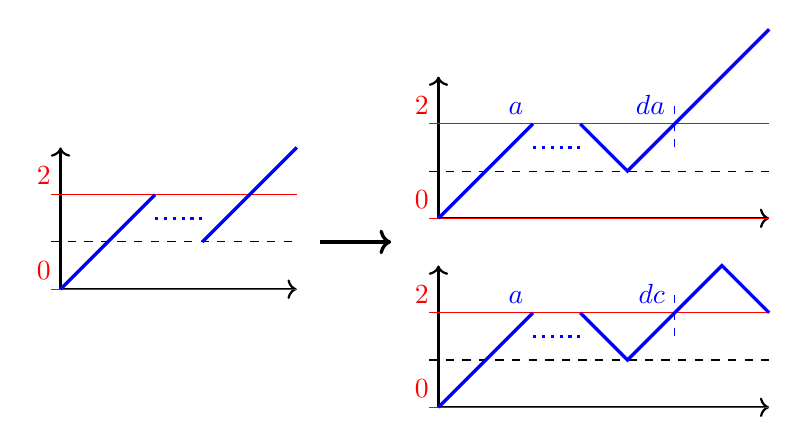
\begin{tikzpicture}[scale=.6]
                \draw[<->, thick] (0, 3) -- (0, 0) -- (5, 0);
                \draw[dashed] (-.2, 1) --(5, 1);
                \draw[red] (-.2, 2) --(5, 2);
                \draw[red] (-.2, 0) --(5, 0);
                \draw[red] (0, 2) node[above left] {2};
                \draw[red] (0, 0) node[above left] {0};
                \draw[blue, very thick] (0, 0) -- (2, 2);
                \draw[blue, very thick, dotted] (2, 1.5) -- (3, 1.5);
                \draw[blue, very thick] (3, 1) -- (5, 3);
                \draw[->, very thick] (5.5, 1) -- (7, 1);

                \draw[<->, thick] (8+0, 3+1.5) -- (8+0, 0+1.5) -- (8+5+2, 0+1.5);
                \draw[dashed] (8+-.2, 1+1.5) --(8+5+2, 1+1.5);
                \draw[red] (8+-.2, 2+1.5) --(8+5+2, 2+1.5);
                \draw[red] (8+-.2, 0+1.5) --(8+5+2, 0+1.5);
                \draw[red] (8+0, 2+1.5) node[above left] {2};
                \draw[red] (8+0, 0+1.5) node[above left] {0};
                \draw[blue, very thick] (8+0, 0+1.5) -- (8+2, 2+1.5);
                \draw[blue, very thick, dotted] (8+2, 1.5+1.5) -- (8+3, 1.5+1.5);
                \draw[blue, very thick] (8+3, 2+1.5) -- (8+4, 1+1.5) -- (8+7, 4+1.5);
                \draw[blue, dashed] (13, 1.5+1.5) -- (13, 4);
                \draw[blue] (13, -.5+4) node[above left] {$da$};
                \draw[blue] (10, -.5+4) node[above left] {$a$};

                \draw[<->, thick] (8+0, 3+1.5-4) -- (8+0, 0+1.5-4) -- (8+5+2, 0+1.5-4);
                \draw[dashed] (8+-.2, 1+1.5-4) --(8+5+2, 1+1.5-4);
                \draw[red] (8+-.2, 2+1.5-4) --(8+5+2, 2+1.5-4);
                \draw[red] (8+-.2, 0+1.5-4) --(8+5+2, 0+1.5-4);
                \draw[red] (8+0, 2+1.5-4) node[above left] {2};
                \draw[red] (8+0, 0+1.5-4) node[above left] {0};
                \draw[blue, very thick] (8+0, 0+1.5-4) -- (8+2, 2+1.5-4);
                \draw[blue, very thick, dotted] (8+2, 1.5+1.5-4) -- (8+3, 1.5+1.5-4);
                \draw[blue, very thick] (8+3, 2+1.5-4) -- (8+4, 1+1.5-4) -- (8+6, 3+1.5-4) -- (8+7, 2+1.5-4);
                \draw[blue, dashed] (13, -1) -- (13, 0);
                \draw[blue] (13, -.5) node[above left] {$dc$};
                \draw[blue] (10, -.5) node[above left] {$a$};

            \end{tikzpicture}
            \caption{Configurations for a $+3$-string of size greater than 3.}
            \label{fig:p3string2piece}
        \end{minipage}
    \end{figure}

    \qed
\end{tproof}
Finally, a word on the alphabet $\mathcal{A}$ embodies a Dyck word of
height at most 2 if and only if it does not contain $aa, ac, bb, bd, cb, cd, da, dc$.
The following \textsc{Algorithm} \autoref{alg:dyck2nsqrt} for \Dyck{2}
comes from the direct application of the theorem.


\begin{algorithm}
    \caption{\textsc{DyckFast}$_{2,n}$}\label{alg:dyck2nsqrt}
    \begin{algorithmic}
        \Require $n \geq 0$, $x$ such that  $|x| = 2n$
        \State $x \gets 11x00$
        \State $\texttt{t} \gets \Null$
        \For{$\texttt{reject\_symbol} \in \{aa, ac, bb, bd, cb, cd, da, dc\}$}
        \If{$t == \Null$}
        \State \textbf{Find} $\texttt{t}$ in $\llbracket0, n\rrbracket$ such that \\
        \hspace*{1cm} $x[2\texttt{t}+1, \ldots, 2\texttt{t}+4] = \texttt{reject\_symbol}$
        \EndIf
        \EndFor
        \State \textbf{return} $\texttt{t} == \Null$

    \end{algorithmic}
\end{algorithm}

\begin{theorem}{\textbf{The quantum query complexity of \textsc{DyckFast}$_{2,n}$.}}
    The \textsc{DyckFast}$_{2,n}$ algorithm has a quantum query complexity of $O\left(\sqrt{n}\right)$.
\end{theorem}

\begin{tproof}
    The algorithm is doing at most 8 Grover's searches on the modified input
    string $11x00$. So the total quantum query complexity is
    \[Q(\textsc{DyckFast}_{2, n}) = 8\times O\left(\sqrt{n+4}\right) = O\left(\sqrt{n}\right).\]

    \qed
\end{tproof}

\subsection{A simplification for \Dyck{2} algorithm}

The algorithm describes in \autoref{subsection:dyck2n} is complex to explain
but it turns out that a simpler version of it exists and is really easier to
understand that the first one.

\begin{algorithm}
    \caption{\textsc{DyckFastEasy}$_{2,n}$}\label{alg:dyck2nsqrteasy}
    \begin{algorithmic}
        \Require $n \geq 0$, $x$ such that  $|x| = 2n$
        \State $x \gets 11x00$
        \State \textbf{Find} $\texttt{t}$ in $\llbracket1, n+1\rrbracket$ such that \\
        \hspace*{1cm} $x[2\texttt{t}, 2\texttt{t}+1] \in \{00, 11\}$
        \State \textbf{return} $\texttt{t} == \Null$
    \end{algorithmic}
\end{algorithm}

Lets explain how it works. A Dyck word of height at most 2 is recognized by
the following grammar on the alphabet $\{0, 1\}$:
\begin{align*}
    S & \mapsto 0I1                             \\
    I & \mapsto 01I \vert 10I \vert \varepsilon \\
\end{align*}
Indeed, a Dyck word of height at most 2 $w_1\ldots w_n$ can only start with
a zero else it gets a negative height. After, if it goes up, it reach the
height 2 so it can only go down. If it goes down instead of going up, it
reaches height 0 so it can only go up. This implies that after every letter
of odd indices, the height is equal to one, and that the next
two letters can only be in $\{01, 10\}$. So, finding a 00, or 11 starting
on an even index is equivalent to not being a dyck word of height at most two.
Finally, it becomes sufficient to use two Grover searches for 00 and 11
in order to recognize \Dyck{2,n}.

\subsection{A final improvement to \Dyck{k} algorithm}

The last algorithm describes is useful to recognize \Dyck{2}. However, it cannot
be plug into the huge one because it does not return the $\pm 3$-string that
allows it to reject. Indeed, the algorithm only finds the second $\pm 2$-string
of the $\pm 3$-string. So,in order to reduce the complexity of the main algorithm,
it is required to find the first  $\pm 2$-string. To do that, it is sufficient
to make a call to the already existing subroutines \FF{2} described in
\autoref{alg:FF} by asking for the closest $\pm 2$-string on the left of the
already known $\pm 2-$string. This is done with a quantum query complexity of
$O(\sqrt{n})$ (Computations are similar to the ones done in the proof in
\autoref{proof:complexity_dyckkn}). Thus, it is easy to modify a little
the algorithm \textsc{DyckFastEasy}{2,n} to return the $\pm 3$-string when
it rejects. Finally, it can be plug into the main algorithm, the computation
of the quantum query complexity are almost identical to the one done in
\autoref{proof:complexity_dyckkn} but initial case is for $k=2$ instead of $k=1$.
The consequence is the removing of a recursion step which implies the loss of
a $\sqrt{\log_2(n)}$ factor which bring the quantum query complexity of
the algorithm that recognizing \Dyck{k} to $O(\sqrt{n}(\log_2(n))^{0.5(k-2)})$.

\section{Conclusion}

Conclusion here.


\bibliographystyle{plain}
\bibliography{biblio}
\listoffigures
\listofalgorithms

\newpage

\section{Appendix}

\begin{appendix}
       \section{Proof of the super-basic adversary method}\label{proof:advmethod}
    As a little reminder here is the theorem.
    \begin{theorem}
        Let define $YES$ the set equal to $f^{-1}(accepted)$ and $NO$ the set
        equal to

        $f^{-1}(rejected)$. If it exist two subset $Y\subseteq YES$ and
        $Z \subseteq NO$ such that:
        \begin{itemize}
            \item For each $y$ in $Y$, there are at least $m$ strings $z$ in $Z$ with dist$(y,z)=1$.
            \item For each $z$ in $Z$, there are at least $m'$ strings $y$ in $Y$ with dist$(y,z)=1$.
        \end{itemize}
        Then the quantum query complexity $Q(f)$ is in  $\Omega(\sqrt{m\times m'})$
    \end{theorem}

    Understanding this proof is important as it gives the intuitions to understand the
    general adversary.

    \begin{tproof}
        First, let's define $\mathcal{R}:= \{(y, z)$ such that $ y \in Y, z \in Z,$ and dist$(y,z)=1\}$.
        Now, it is necessary to redefine the progress notion such that
        $\mathcal{P}(t) := \sum_{(y,z) \in \mathcal{R}}\vert \langle \psi^t_y \vert \psi^t_z \rangle\vert$
        where $\ket{\psi_x^t}$ is the state of the algorithm after $t$ query to the entry $x$.
        So, $\mathcal{P}(0) = \vert \mathcal{R} \vert$ and $\mathcal{P}(T) = \vert \frac{2}{3}\mathcal{R} \vert$.
        In order to prove the theorem, lets try to prove that for all $t$,
        \[\mathcal{P}(t) - \mathcal{P}(t+1) \leq \frac{2}{\sqrt{m m'}}\vert \mathcal{R}\vert\]
        as it is a correct value
        of $d$ such that the lower bound is $O(\sqrt{mm'})$. Moreover, there are relations between sizes
        of the sets:
        \[\vert \mathcal{R} \vert \geq m \vert Y \vert, \vert \mathcal{R} \vert \geq m' \vert Z \vert
            \implies \vert 2\mathcal{R} \vert \geq m \vert Y \vert+ m' \vert Z \vert.\] Thus, instead of proving
        $\mathcal{P}(t) - \mathcal{P}(t+1) \leq \frac{2}{\sqrt{m m'}}\vert \mathcal{R}\vert$, lets try
        to prove
        \[\mathcal{P}(t) - \mathcal{P}(t+1) \leq \frac{1}{\sqrt{m m'}}(m \vert Y \vert+ m' \vert Z \vert)
            = \sqrt{\frac{m}{m'}} \vert Y \vert + \sqrt{\frac{m'}{m}}\vert Z \vert.\]
        Now, lets take any a couple $(y,z)$ in $\mathcal{R}$, it exists a unique $i^*$ such that $y_{i^*} \neq z_{i^*}$.
        This small variation between $y$ and $z$ can be well translated to the progress after quantum query gate.
        Lets write $\ket{\psi^{t}_y}$ and $\ket{\psi^{t}_z}$: \\
        \[\ket{\psi^{t}_y} = \sum_{\substack{i \in \llbracket0,N\rrbracket\\j \in \llbracket1, d_i\rrbracket}}\alpha_{i,j} \ket{i,j} \hspace*{3cm }
            \ket{\psi^{t}_z} = \sum_{\substack{i \in \llbracket0,N\rrbracket\\j \in \llbracket1, d_i\rrbracket}}\beta_{i,j} \ket{i,j}.\]
        Now by applying $Q_t$, the states become
        \[\ket{\psi^{t}_y} = \sum_{\substack{i \in \llbracket0,N\rrbracket\\j \in \llbracket1, d_i\rrbracket}} (-1)^{(0y)_{i+1}}\alpha_{i,j} \ket{i,j} \hspace*{1cm }
            \ket{\psi^{t}_z} = \sum_{\substack{i \in \llbracket0,N\rrbracket\\j \in \llbracket1, d_i\rrbracket}}(-1)^{(0z)_{i+1}}\beta_{i,j} \ket{i,j}.\]
        However, $y$ and $z$ only differ on the index $i^*$, so the restricted progress measure
        to $y$ and $z$ at $t$ and $t+1$ are equal to
        \begin{align*}
            \mathcal{P}_{y,z}(t) = \sum_{\substack{i \in \llbracket0,N\rrbracket                        \\j \in \llbracket1, d_i\rrbracket}} \overline{\alpha_{i,j}}\beta_{i,j} \hspace*{1cm}
            \mathcal{P}_{y,z}(t+1) & = \sum_{\substack{i \in \llbracket0,N\rrbracket                    \\j \in \llbracket1, d_i\rrbracket}} (-1)^{(0y)_{i+1}+(0z)_{i+1}} \overline{\alpha_{i,j}}\beta_{i,j} \\
                                   & = \sum_{\substack{i \in \llbracket0,N\rrbracket                    \\j \in \llbracket1, d_i\rrbracket}} \overline{\alpha_{i,j}}\beta_{i,j} -
            2\sum_{j\in\llbracket1,d_{i^*}\rrbracket} \overline{\alpha_{i^*,j}}\beta_{i^*,j}            \\
                                   & = \mathcal{P}_{y,z}(t) - 2\sum_{j\in\llbracket1,d_{i^*}\rrbracket}
            \overline{\alpha_{i^*,j}}\beta_{i^*,j}       .                                              \\
        \end{align*}
        So, for restricted progress measures there is the inequality
        \begin{align*}
            \vert \mathcal{P}_{y,z}(t)\vert - \vert \mathcal{P}_{y,z}(t+1)\vert & \leq \vert \mathcal{P}_{y,z}(t) - \mathcal{P}_{y,z}(t+1)\vert                                      \\
                                                                                & \leq \vert 2\sum_{j\in\llbracket1,d_{i^*}\rrbracket} \overline{\alpha_{i^*,j}}\beta_{i^*,j}  \vert \\
                                                                                & \leq 2\sum_{j\in\llbracket1,d_{i^*}\rrbracket} \vert\alpha_{i^*,j}\vert\vert\beta_{i^*,j}\vert.
        \end{align*}
        Moreover, the math trick for all $p$, $q$ real numbers and $h$ non negative real number
        $2pq \leq hp^2 + \frac{1}{h}q^2 $ allow to rewrite the previous inequality to
        \begin{align*}
            \vert \mathcal{P}_{y,z}(t)\vert - \vert \mathcal{P}_{y,z}(t+1)\vert & \leq 2\sum_{j\in\llbracket1,d_{i^*}\rrbracket}  \vert\alpha_{i^*,j}\vert\vert\beta_{i^*,j}\vert                                             \\
                                                                                & \leq \sum_{j\in\llbracket1,d_{i^*}\rrbracket} h\vert\alpha_{i^*,j}\vert^2 + \frac{1}{h}\vert\beta_{i^*,j}\vert^2.                           \\
            \intertext{By chosing $h$ equal to $\sqrt{\frac{m}{m'}}$, it becomes}
            \vert \mathcal{P}_{y,z}(t)\vert - \vert \mathcal{P}_{y,z}(t+1)\vert & \leq \sum_{j\in\llbracket1,d_{i^*}\rrbracket} \sqrt{\frac{m}{m'}}\vert\alpha_{i^*,j}\vert^2 + \sqrt{\frac{m'}{m}}\vert\beta_{i^*,j}\vert^2. \\
        \end{align*}
        Now, it is time to sum on every couple $(y,z)$ of $\mathcal{R}$. But $i^*$ is depending on $y,z$ as much
        as $\alpha_{i,j}$s and $\beta_{i,j}$s so lets give them $y$ and $z$ as argument

        \begin{align*}
            \mathcal{P}(t)- \mathcal{P}(t+1) & = \sum_{(y,z)\in\mathcal{R}} \left\vert\mathcal{P}_{y,z}(t)\right\vert - \sum_{(y,z)\in\mathcal{R}} \left\vert\mathcal{P}_{y,z}(t+1)\right\vert         \\
                                             & \leq \sum_{\begin{matrix}
                    (y,z) \in \mathcal{R} \\
                    j\in\llbracket1,d_{i^*_{y,z}}\rrbracket
                \end{matrix}} \sqrt{\frac{m}{m'}}\vert\alpha^{y}_{i^*_{y,z},j}\vert^2 + \sqrt{\frac{m'}{m}}\vert\beta^{z}_{i^*_{y,z},j}\vert^2. \\
        \end{align*}
        Now, it is useful to do the first summation in two part in order to find a upped bound to the sum
        \begin{align*}
            \mathcal{P}(t)- \mathcal{P}(t+1)  \leq & \sqrt{\frac{m}{m'}}
            \sum_{\substack{y\ st\ \exists z                                                               \\ (y,z) \in \mathcal{R}}}
            \sum_{\substack{z\ \textrm{width}                                                              \\ (y,z) \in \mathcal{R}}}
            \sum_{j\in\llbracket1,d_{i^*_{y,z}}\rrbracket}\vert\alpha^{y}_{i^*_{y,z},j}\vert^2             \\
                                                   & +\sqrt{\frac{m'}{m}} \sum_{\substack{z\ st\ \exists y \\ (y,z) \in \mathcal{R}}}
            \sum_{\substack{y\ \textrm{width}                                                              \\ (y,z) \in \mathcal{R}}}
            \sum_{j\in\llbracket1,d_{i^*_{y,z}}\rrbracket}\vert\beta^{z}_{i^*_{y,z},j}\vert^2.
        \end{align*}
        Now, at $y$ fixed, $z \mapsto i^*_{y,z}$ is an injective function from $\{z, (y,z)\in \mathcal{R\}}$ to $\llbracket1, N\rrbracket$ as
        $y$ and $z$ are at distance 1. Thus $(z,j) \mapsto (i^*_{y,z}, j)$ is also an injective function
        from $\{(z,j), (y,z)\in \mathcal{R}\ \textrm{and}\ j \in \llbracket1, d_{i^*_{y,z}}\rrbracket\}$ to
        $\llbracket1, N\rrbracket\times\llbracket1, d_{i^*_{y,z}}\rrbracket$.
        So, it implies that
        \[ \bigsqcup_{\substack{z\ \textrm{width}\\ (y,z) \in \mathcal{R}}} \{i^*_{y,z}\}\times \llbracket 1,d_{i^*_{y,z}}\rrbracket\subseteq \bigsqcup_{n \in \llbracket0,N\rrbracket} \{n\}\times\llbracket1,d_n\rrbracket\]
        and finally that
        \begin{align*}
            \sum_{\substack{z\ \textrm{width} \\ (y,z) \in \mathcal{R}}}
            \sum_{j\in\llbracket1,d_{i^*_{y,z}}\rrbracket}\vert\alpha^{y}_{i^*_{y,z},j}\vert^2
            \leq \sum_{i \in \llbracket0,N\rrbracket}
            \sum_{j\in\llbracket1,d_{i}\rrbracket}\vert\alpha^{y}_{i,j}\vert^2 \leq \left\langle \psi_y^t \vert \psi_y^t \right\rangle \leq 1.
        \end{align*}
        By symmetry it also works for the second sum, so the difference of progress is now the following
        \begin{align*}
            \mathcal{P}(t)- \mathcal{P}(t+1)  \leq & \sqrt{\frac{m}{m'}}
            \sum_{\substack{y\ st\ \exists z                                                                               \\ (y,z) \in \mathcal{R}}}
            \sum_{\substack{z\ \textrm{width}                                                                              \\ (y,z) \in \mathcal{R}}}
            \sum_{j\in\llbracket1,d_{i^*_{y,z}}\rrbracket}\vert\alpha^{y}_{i^*_{y,z},j}\vert^2                             \\
                                                   & +\sqrt{\frac{m'}{m}} \sum_{\substack{z\ st\ \exists y                 \\ (y,z) \in \mathcal{R}}}
            \sum_{\substack{y\ \textrm{width}                                                                              \\ (y,z) \in \mathcal{R}}}
            \sum_{j\in\llbracket1,d_{i^*_{y,z}}\rrbracket}\vert\beta^{z}_{i^*_{y,z},j}\vert^2                              \\
            \leq                                   & \sqrt{\frac{m}{m'}} \sum_{\substack{y\ st\ \exists z                  \\ (y,z) \in \mathcal{R}}} 1 + \sqrt{\frac{m'}{m}} \sum_{\substack{z\ st\ \exists y \\ (y,z) \in \mathcal{R}}} 1 \\
            \leq                                   & \sqrt{\frac{m}{m'}} \vert Y \vert + \sqrt{\frac{m'}{m}} \vert Z \vert \\
            \leq                                   & \frac{2}{\sqrt{mm'}}\vert \mathcal{R} \vert.
        \end{align*}
        To conclude, it gives a lower bound $\Omega(\sqrt{mm'})$ for the quantum query complexity of $f$.

        \qed

    \end{tproof}

    \newpage

    \section{The algorithm for \Dyck{k, n}}
    \label{annex:complete_subroutine_dyck_kn}
    All the subroutines' pseudo codes can be found from \textsc{Algorithm}
    \autoref{alg:dyck_kn} to \textsc{Algorithm} \autoref{alg:ffp}.

    \begin{algorithm}[h!]
        \caption{\Dyck{k,n}}\label{alg:dyck_kn}
        \begin{algorithmic}
            \Require $n \geq 0$ and $k \geq 1$
            \Ensure $|x| = n $
            \State $x \gets 1^kx0^k$
            \State $v \gets$ \FA{k+1}$(0, n+2*k-1, \{1,-1\})$
            \State \textbf{return} v = \Null
        \end{algorithmic}
    \end{algorithm}

    \begin{algorithm}[h!]
        \caption{\FA{k}$(l,r,s)$}\label{alg:fa_k}
        \begin{algorithmic}
            \Require $0 \leq l < r$ and $s \subseteq \{1,-1\}$
            \State \textbf{Find} $d$ in $\{2^{\lceil \log_2(k)\rceil }, 2^{\lceil \log_2(k)+1\rceil },\ldots,2^{\lceil \log_2(r-l)\rceil }\}$
            such that \\
            \hspace*{1cm} $v_d \gets $ \FFL{k}$(l,r,d,s)$ is \textbf{not} \Null
            \State \textbf{return} $v_d$ or \Null \ if none
        \end{algorithmic}
    \end{algorithm}

    \begin{algorithm}[h!]
        \caption{\FFL{k}$(l,r,d,s)$}\label{alg:ffl_k}
        \begin{algorithmic}
            \Require $0 \leq l < r$, $1\leq d \leq r-l$ and $s \subseteq \{1,-1\}$
            \State \textbf{Find} $t$ in $\{l, l+1, \dots, r\}$ such that \\
            \hspace*{1cm} $v_t \gets$ \FALM{k}$(l,r,t,d,s)$ is \textbf{not} \Null
            \State \textbf{return} $v_t$ of \Null if none
        \end{algorithmic}
    \end{algorithm}

    \begin{algorithm}[h!]
        \caption{\FALM{k}$(l,r,d,t,s)$}\label{alg:falm_k}
        \begin{algorithmic}
            \Require $0 \leq l < r$, $l \leq r \leq r$, $1\leq d \leq r-l$ and $s \subseteq \{1,-1\}$
            \State $v = (i_1,j_1,\sigma_1) \gets \FALM{k-1}(l,r,t,d-1,\{1,-1\})$
            \If{$v \neq \Null$} {
                \State $v' = (i_2,j_2,\sigma_2) \gets \FARM{k-1}(l,r,i_1-1,d-1,\{1,-1\})$
                \If{$v' = \Null$}
                \State $v' = (i_2,j_2,\sigma_2) \gets \FF{k-1}(\max(l, j_1-d+1),i_1-1,\{1,-1\}, left)$
                \EndIf
                \If{$v'\neq \Null$ and $\sigma_2 \neq \sigma_1$}{\ $v' \gets \Null$}
                \EndIf
                \If{$v' = \Null$}
                \State $v' = (i_2,j_2,\sigma_2) \gets \FALM{k-1}(l,r,j_1+1,d-1,\{1,-1\})$
                \EndIf
                \If{$v' = \Null$}
                \State $v' = (i_2,j_2,\sigma_2) \gets \FF{k-1}(j_1+1,\max(r, i_1+d-1),\{1,-1\}, right)$
                \EndIf
                \If{$v' = \Null$}{\ \textbf{return} \Null}
                \EndIf
            }
            \Else {
            \State $v = (i_1,j_1,\sigma_1) \gets \FF{k-1}(t, min(t+d-1, r), \{1,-1\}, right)$
            \If{v = \Null}{\ \textbf{return} \Null}
            \EndIf
            \State $v' = (i_2, j_2, \sigma_2) \gets \FF{k-1}(max(t-d+1, l), t, \{1, -1\}, left)$
                \If{$v' = \Null$}{\ \textbf{return} \Null}
                \EndIf
                }
                \EndIf
                \If{$\sigma_1=\sigma_2$ and $\sigma_1 \in s$ and $\max(j_1, j_2) - \min(i_1, i_2) + 1 \leq d$}
                \State \textbf{return} $(\min(i_1, i_2), \max(j_1, j_2), \sigma_1)$
            \Else{\ \textbf{return} \Null}
            \EndIf

        \end{algorithmic}
    \end{algorithm}

    \begin{algorithm}[h!]
        \caption{\FF{k}$(l, r, s, left)$}
        \label{alg:FF}
        \begin{algorithmic}
            \Require $0\leq l < r$ and $s \subseteq \{1,-1\}$
            \State $lBorder \gets l, rBorder \gets r, d \gets 1$
            \While{$lBorder + 1 < rBorder $}
            \State $ mid \gets \lfloor (lBorder + rBorder)/2 \rfloor $
            \State $v_l \gets \FA{k}(lBorder, mid, s)$
            \If{$v_l \neq \Null$}{\ $rBorder \gets mid$}
            \Else
            \State $v_{mid} \gets \FFP{k}(lBorder, rBorder, mid, s, left)$
            \If{$v_{mid} \neq \Null$}{\ \textbf{return} $v_{mid}$}
            \Else{\ $lBorder \gets mid + 1$}
            \EndIf
            \EndIf
            \State $d \gets d+1$
            \EndWhile
            \State \textbf{return} \Null
        \end{algorithmic}
    \end{algorithm}


    \begin{algorithm}[h!]
        \caption{$\FFP{k}(l,r,t,s)$}\label{alg:ffp}
        \begin{algorithmic}
            \Require $0\leq l<r$, $l \leq t \leq r$ and $s \subseteq \{1, -1\}$

            \State \textbf{Find} $d$ in $\{2^{\lceil \log_2(k)\rceil }, 2^{\lceil \log_2(k)+1\rceil },\ldots,2^{\lceil \log_2(r-l)\rceil }\}$
            such that \\
            \hspace*{1cm} $v_d \gets $ \FALM{k}$(l,r,t,d,s)$ is \textbf{not} \Null
            \State \textbf{return} $v_d$ or \Null \ if none
        \end{algorithmic}
    \end{algorithm}

    \newpage

    \section{The proof of the quantum query complexity for \Dyck{k,n} algorithm's subroutines}
    \label{proof:complexity_dyckkn}

    \begin{theorem}{\textbf{\Dyck{k,n}'s Subroutines complexity}}
        The subroutines' quantum query complexity for $k$ are the following.
        \begin{enumerate}
            \item $Q$(\Dyck{k,n}) = $O\left(\sqrt{n}(\log_2(n))^{0.5(k-1)}\right)$ \ for $k \geq 1$
            \item $Q$(\FA{k+1}$(l,r,s)$) = $O\left(\sqrt{r-l}(\log_2(r-l))^{0.5(k-1)}\right)$ \ for $k \geq 1$
            \item $Q$(\FFL{k+1}$(l,r,d,s)$) = $O\left(\sqrt{r-l}(\log_2(r-l))^{0.5(k-2)}\right)$ \ for $k \geq 2$
            \item $Q$(\FALM{k+1}$(l, r, t, d, s)$) = $\left\{
                      \begin{array}{ll}
                          O\left(\sqrt{d}(\log_2(d))^{0.5(k-2)}\right) & \textrm{for} \ k \geq 2 \\
                          O(1)                                         & \textrm{for} \  k = 1
                      \end{array}
                      \right.$
            \item $Q$(\FF{k}$(l,r,s, left)$) = $O\left(\sqrt{r-l}(\log_2(r-l))^{0.5(k-2)}\right)$ \ for $k \geq 2$
            \item $Q$(\FFP{k}$(l,r,t,s)$) = $\left\{ \begin{array}{ll}
                          O\left(\sqrt{r-l}(\log_2(r-l))^{0.5(k-2)}\right) & \textrm{for} \ k \geq 3 \\
                          O(1)                                             & \textrm{for} \ k = 2
                      \end{array}
                      \right.$
        \end{enumerate}
    \end{theorem}

    \begin{tproof} The proof is done by induction on the height $k$ of the Dyck word.
        \init{For $k=1$ and $k=2$ we have the following initialization. \\
            \begin{itemize}
                \item For $k=1$, only \FALM{2}, \FA{2} ,and \Dyck{1,n} are defined. The $O(1)$ quantum query complexity
                      of \FALM{2} comes directly from the definition of its initial case, as the $O(\sqrt{r-l})$ quantum
                      query complexity of \FA{2}. Then the $O\left(\sqrt{n}\right)$ quantum query complexity of \Dyck{1,n} comes from
                      the call to \FA{2}.
                \item For $k=2$, the inductive part of the algorithm starts and every subroutines is defined. The $O(1)$
                      quantum query complexity of \FFP{2} comes from the call to \FALM{2}.
                      The $O\left(\sqrt{r-l}\right)$ quantum query complexity of \FF{2} comes from the dichotomize search using \FA{2} and
                      \FFP{2} because $\sum_{u=1}^{log_2(r-l)}2u\left(O\left(\sqrt{\frac{r-l}{2^{u-1}}}\right)+O(1)\right) = O(\sqrt{r-l})$
                      (Detailed in the induction). The $O(\sqrt{d})$ quantum query complexity of \FALM{3} comes from the
                      constant amount of calls to \FF{2} and \FALM{2} with entry of size $d$. The $O(\sqrt{r-l})$ quantum query
                      complexity of \FFL{3} comes from the $O\left(\sqrt{\frac{r-l}{d}}\right)$ calls to \FALM{3}. The $O\left(\sqrt{(r-l)\log_2(r-l)}\right)$
                      quantum query complexity of \FA{3} comes from the $O\left(\sqrt{\log_2(r-l)}\right)$ calls to \FFL{3}. Finally, the
                      $O\left(\sqrt{(r-l)\log_2(r-l)}\right)$ quantum query complexity of \Dyck{2} comes from the call to \FA{3}.
            \end{itemize}
        }
        \hered{Lets suppose it exists $k$ such that \autoref{th:subroutine_complexity} is
            true for $k$. Lets prove that it is true for $k+1$. \\

            First, the $O\left(\sqrt{r-l}(\log_2(r-l))^{0.5(k-1)}\right)$ quantum query complexity of \FFP{k+1} comes from
            the $O\left(\sqrt{\log(r-l)}\right)$ calls to \FALM{k+1}.
            \begin{align*}
                Q(\textrm{\FFP{k+1}}(l, r, t, s)) & = O(\sqrt{\log(r-l)}) \times O\left(Q(\textrm{\FALM{k+1}}(l, r, t, d, s))\right)\            \\
                                                  & \overset{IH}{=} O \left( \sqrt{\log(r-l)} \times \sqrt{r-l}(\log_2(r-l))^{0.5(k-2)}  \right) \\
                                                  & = O \left( \sqrt{r-l}(\log_2(r-l))^{0.5(k-1)} \right)
            \end{align*}

            Thus the $O \left(\sqrt{r-l}(\log_2(r-l))^{0.5(k-2)}\right)$ quantum query complexity of \FF{k+1} comes
            from the dichotomize search using calls to \FA{k+1} and \FF{k+1}.

            \blfootnote{\begin{align*}
                    ^{a}\sum_{u=1}^{+\infty} \left(\frac{\textrm{d}}{\textrm{d}x}(x^{u})\right)\left(\frac{1}{\sqrt{2}}\right)
                    \leq \left(\frac{\textrm{d}}{\textrm{d}x} \left( \sum_{u=1}^{+\infty} x^u \right)\right)\left(\frac{1}{\sqrt{2}}\right)
                    \leq \left(\frac{\textrm{d}}{\textrm{d}x} \left( \frac{x}{1-x} \right)\right)\left(\frac{1}{\sqrt{2}}\right)
                    \leq \left(\frac{1}{(1-x)^2}\right)\left(\frac{1}{\sqrt{2}}\right)
                    \leq \frac{1}{(1-\frac{1}{\sqrt{2}})^2} \leq \frac{\sqrt{2}^2}{(\sqrt{2} - 1)^2}
                \end{align*}}

            \begin{align*}
                Q(\textrm{\FF{k+1}}(l,r,t,d,s)) & = \begin{array}{l}
                    \sum_{u=1}^{\log_2(r-l)}2u \times O\left(Q(\textrm{\FA{k+1}}(0, \frac{r-l}{2^{u-1}}, s))\right) \\
                    + \sum_{u=1}^{\log_2(r-l)}2u \times O\left(Q(\textrm{\FFP{k+1}}(0, \frac{r-l}{2^{u-1}}, \_ , s, left))\right)
                \end{array}                                                     \\
                                                & \overset{IH}{=}
                O\left(\sum_{u=1}^{\log_2(r-l)}2u \times \sqrt{\frac{r-l}{2^{u-1}}}(\log_2(\frac{r-l}{2^{u-1}}))^{0.5(k-1)}\right) \\
                                                & =
                O\left(\sum_{u=1}^{\log_2(r-l)}2u \times \sqrt{\frac{r-l}{2^{u-1}}}(\log_2(r-l))^{0.5(k-1)}\right)                 \\
                                                & =
                O \left(\sqrt{r-l}(\log_2(r-l))^{0.5(k-1)}\sum_{u=1}^{\log_2(r-l)}u\times (\frac{1}{\sqrt{2}})^{u-1} \right)       \\
                                                & =^{a}
                O \left(\sqrt{r-l}(\log_2(r-l))^{0.5(k-1)} \frac{\sqrt{2}^2}{(\sqrt{2}-1)^2}\right)                                \\
                                                & =
                O \left(\sqrt{r-l}(\log_2(r-l))^{0.5(k-1)}\right)
            \end{align*}


            Next, the $ O\left(\sqrt{d}(\log_2(d))^{0.5(k-1)} \right)$ quantum query complexity comes of \FALM{k+2}from the constant amount
            of calls to \FALM{k+1}, \FARM{k+1} ,and \FF{k+1}.

            \begin{align*}
                Q(\textrm{\FALM{k+2}}(l,r,t,d,s)) & = \begin{array}{l}
                    3 \times O\left(Q(\textrm{\FALM{k+1}}(l,r,t,d,\{1,-1\}))\right) \\
                    + 4 \times O\left(Q(\textrm{\FF{k+1}}(l,r,\{1,-1\},left))\right)
                \end{array}                                  \\
                                                  & \overset{IH}{=} O\left(\sqrt{d}(\log_2(d))^{0.5(k-1)} \right)
            \end{align*}

            After that, the $O\left( \sqrt{r-l}(\log_2(r-l))^{0.5(k-1)}\right)$ quantum query complexity of \FFL{k+2} comes from the
            $O\left(\sqrt{\frac{r-l}{d}}\right)$ calls to \FALM{k+2}.

            \begin{align*}
                Q(\textrm{\FFL{k+2}}(l, r, d, s)) & = O\left(\sqrt{\frac{r-l}{d}}\right) \times O\left(Q(\textrm{\FALM{k+2}}(l,r,t,d,s))\right) \\
                                                  & = O\left( \sqrt{\frac{r-l}{d}} \times \sqrt{d}(\log_2(d))^{0.5(k-1)}\right)                 \\
                                                  & = O\left( \sqrt{r-l}(\log_2(d))^{0.5(k-1)}\right)                                           \\
                                                  & = O\left( \sqrt{r-l}(\log_2(r-l))^{0.5(k-1)}\right)
            \end{align*}

            Hence, the $O\left( \sqrt{r-l}(\log_2(r-l))^{0.5k} \right)$ quantum query complexity of \FA{k+2} comes from
            the $O\left(\sqrt{\log_2(r-l)}\right)$ calls to \FFL{k+2}.

            \begin{align*}
                Q(\textrm{\FA{k+2}}(l, r, s)) & = O\left(\sqrt{\log(r-l)}\right) \times O\left(Q(\textrm{\FFL{k+2}}(l, r, d, s))\right) \\
                                              & = O\left( \sqrt{\log(r-l)} \times \sqrt{r-l}(\log_2(r-l))^{0.5(k-1)} \right)            \\
                                              & = O\left( \sqrt{r-l}(\log_2(r-l))^{0.5k} \right)                                        \\
            \end{align*}

            Finally, the $O\left( \sqrt{n}(\log_2(n))^{0.5k} \right)$ quantum query complexity of \Dyck{k+1,n} comes from the
            call to \FA{k+2}.

            \begin{align*}
                Q(\textrm{\Dyck{k+1,n}}) & = O\left(Q(\textrm{\FA{k+2}}(0,n+2k+1,s))\right) \\
                                         & = O\left(Q(\textrm{\FA{k+2}}(0, n, s))\right)    \\
                                         & = O\left( \sqrt{n}(\log_2(n))^{0.5k} \right)
            \end{align*}

        }

        \Conc{By the induction principle,  the \autoref{th:subroutine_complexity} is true for $k \in \mathbb{N}^*$}

        \qed
    \end{tproof}

\end{appendix}


\end{document}